\documentclass[a4paper]{article}

\title{Protein HMM}
\author{Danilo Horta}
\date{August 2019}

\usepackage{natbib}
\usepackage{graphicx}
\usepackage{amsmath}
\usepackage{amsthm}
\usepackage{amssymb}
\usepackage[margin=0.5in]{geometry}
\usepackage{rotating}
\usepackage{subcaption}
\usepackage[T1]{fontenc}

\theoremstyle{definition}
\newtheorem{example}{Example}[section]

\theoremstyle{definition}
\newtheorem{definition}{Definition}[section]

\theoremstyle{definition}
\newtheorem{corollary}{Corollary}[section]

\newcommand{\prob}[1]{p (#1)}
\newcommand{\cprob}[2]{p\left(#1\;\middle|\; #2\right)}
\newcommand{\eps}{\epsilon}
\newcommand{\s}{\texttt{\char`_}}
\newcommand{\gv}{\;|\;}
\newcommand*{\field}[1]{\mathbb{#1}}%

\begin{document}

\maketitle

\section{Model}

\begin{definition}\label{def:hmm}
Let $\mathcal A$ be a finite set of symbols.
Let $Q_1, Q_2, \dots$ be a Markov process and let $S_1, S_2, \dots$ be a stochastic process for which
$p(S_t\in\mathcal A\gv Q_1=q_1, Q_2=q_2, \dots, Q_t=q_t) = p(S_t\in\mathcal A\gv Q_t=q_t)$.
The pair $(Q_t, S_t)$ is a hidden Markov model (HMM) with alphabet $\mathcal A$.
\end{definition}

Let $(Q_t, S_t)$ be a HMM with the amino acid alphabet $\mathcal A$.
We want to replace it with a HMM that generates sequences of symbols from the alphabet
$\mathcal B = \{\mathrm A, \mathrm C, \mathrm G, \mathrm T\}$ of DNA bases and is able to account
for frame-shifting.
Let $\mathrm M_j$ be the so-called match state of an amino acid HMM and let $Q_t=\mathrm M_j$.
From the amino acid emission probabilities and any other relevant source of information
(codon usage bias, for instance), one can define the probability $\cprob{X_1=x_1, X_2=x_2, X_3=x_3}{Q_t=\mathrm M_j}$
of $\mathrm M_j$ emitting the codon $(x_1, x_2, x_3) \in \mathcal B^3$
--- one can also write $\cprob{X=x_1x_2x_3}{Q_t=\mathrm M_j}$, for short.
Since measurement errors occur and nature is not perfect, we will replace the
codon emission process by one that instead produces base sequences of different
lengths to account for base insertions and deletions (indels).

Node $\mathrm M_j$ in Fig.~\ref{fig:codon-hmm-tree} represents the modified match state.
The generated codon will go through four transitions, each one representing one of three possibilities: (i) delete a base; (ii) insert a base; or (iii) do nothing.
The deletion can happen in any of the three codon positions with equal probability.
If a deletion has already happened, the next deletion can happen in any of the remaining two positions with equal probability.
The insertion can happen between any two bases, before the first base or after the last base with equal probability.

The codon emitted at node $\mathrm M_j$ can go under $m\in\{0, 1, 2, 3, 4\}$ base indels during
the state transitions that end at some leaf-node state.
The probability of it undergoing $m$ indels is given by
\begin{align*}
    p(M=m) = \binom{4}{4-m} (1 - \eps)^{4-m} \eps^m,
\end{align*}
where coefficient $\binom{4}{m}$ counts the number of paths corresponding to $m$ base indels.
Fig.~\ref{fig:indel-dist} shows the base indel distributions over different values of $\eps$.
Let $F$ be a random variable representing the final sequence length generated by the model in
Fig.~\ref{fig:codon-hmm-tree}.
We have the probabilities
\begin{align*}
    p(F=1) = p(F=5) &= \eps^2(1-\eps)^2, \\
    p(F=2) = p(F=4) &= 2\eps^3(1-\eps) + 2\eps(1-\eps)^3,~\text{and} \\
    p(F=3)          &= \eps^4 + 4\eps^2(1-\eps)^2 + (1-\eps)^4
\end{align*}
illustrated in Fig.~\ref{fig:len-dist} over different values of $\eps$.

\begin{figure}[htbp]
\centering
\begin{subfigure}{.5\textwidth}
  \centering
  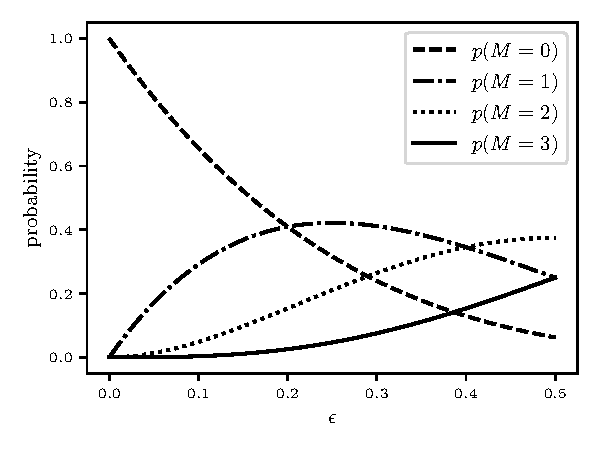
\includegraphics[width=.7\linewidth]{indel-prob}
  \caption{Base indel distribution.}%
  \label{fig:indel-dist}
\end{subfigure}%
\begin{subfigure}{.5\textwidth}
  \centering
  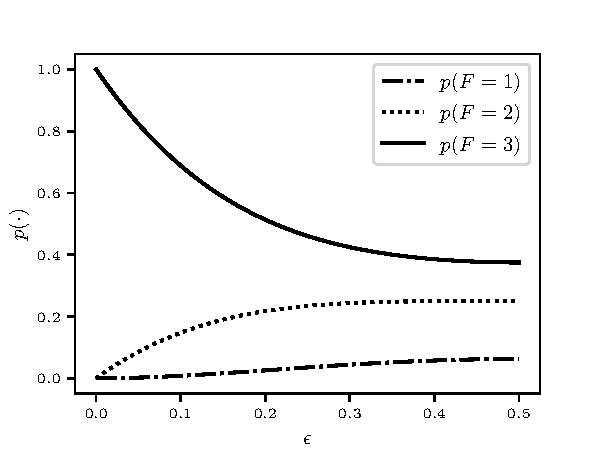
\includegraphics[width=.7\linewidth]{seq-len-prob}
  \caption{Sequence length distribution.}%
  \label{fig:len-dist}
\end{subfigure}
\caption{
    Distribution of base indels and sequence length over the transition probability $\eps$.
    It is recommended to choose a value for $\eps$ that is smaller than $1/5$ such that
    $p(M=m)<p(M=m+1)$, as per Fig.~\ref{fig:indel-dist}.
}
\label{fig:dist}
\end{figure}

A sequence $\mathbf z=z_1 z_2\dots$ of finite but variable length will emerge at the end of the
process represented in Fig.~\ref{fig:codon-hmm-tree}.
Let $\mathcal Q_f$ be the set of hidden paths, starting with $Q_t=\mathrm M_j$ and ending at some leaf-node state,
that generate sequences of length $f$.
Let $Z^f=(Z^f_1, \dots, Z^f_f)$ be a $f$-tuple of random variables that generates such sequences of length $f$.
We have
\begin{align*}
    p(Z^f=z_1\dots z_f,F=f) &= \sum_{\mathbf q \in \mathcal Q_f}
    \cprob{Z^f=z_1\dots z_f}{Q_{t..t+4}=\mathbf q} p(Q_{t..t+4}=\mathbf q).
\end{align*}

\section{Final sequence distribution}

We will write $p(X=x_1x_2x_3) = p(X=x_1x_2x_3 \gv Q_t = \mathrm M_j)$ for brevity.
Underscore $\s$ denotes a summation over the corresponding random variables.
For example, $p(X=x_1\s\s)=\sum_{x_2,x_3}p(X=x_1x_2x_3)$.

\subsection{Sequences of length 1}

\begin{align*}
    p(Z^1=z_1,F=1)
        &= \eps^2(1-\eps)^2(p(X=z_1\s\s) + p(X=\s z_1\s) + p(X=\s\s z_1)) / 3
\end{align*}

\subsection{Sequences of length 2}

\begin{align*}
    p(Z^2=z_1z_2,F=2)
        &= 2\eps(1-\eps)^3(p(X=\s z_1z_2) + p(X=z_1\s z_2) + p(X=z_1z_2\s))/3\\
        &+ \eps^3(1-\eps)(p(X=z_1\s\s) + p(X=\s z_1\s) + p(X=\s\s z_1))p(z_2)/3\\
        &+ \eps^3(1-\eps)(p(X=z_2\s\s) + p(X=\s z_2\s) + p(X=\s\s z_2))p(z_1)/3
\end{align*}

\subsection{Sequences of length 3}

\begin{align*}
    p(Z^3=z_1z_2z_3,F=3) &= (1-\eps)^4 p(X=z_1z_2z_3)\\
        &+ 4\eps^2(1-\eps)^2 (p(X=\s z_2 z_3) + p(X=z_2\s z_3) + p(X=z_2 z_3\s))p(z_1)/9\\
        &+ 4\eps^2(1-\eps)^2 (p(X=\s z_1 z_3) + p(X=z_1\s z_3) + p(X=z_1 z_3\s))p(z_2)/9\\
        &+ 4\eps^2(1-\eps)^2 (p(X=\s z_1 z_2) + p(X=z_1\s z_2) + p(X=z_1 z_2\s))p(z_3)/9\\
        &+ \eps^4 (p(X=z_3\s\s) + p(X=\s z_3\s) + p(X=\s\s z_3))p(z_1)p(z_2)/9\\
        &+ \eps^4 (p(X=z_2\s\s) + p(X=\s z_2\s) + p(X=\s\s z_2))p(z_1)p(z_3)/9\\
        &+ \eps^4 (p(X=z_1\s\s) + p(X=\s z_1\s) + p(X=\s\s z_1))p(z_2)p(z_3)/9
\end{align*}

\subsection{Sequences of length 4}

\begin{align*}
    p(Z^4=z_1z_2z_3z_4,F=4) &= \eps(1-\eps)^3 (p(X=z_2z_3z_4)p(z_1)+p(X=z_1z_3z_4)p(z_2)\\
        &+p(X=z_1z_2z_4)p(z_3)+p(X=z_1z_2z_3)p(z_4))/2\\
        &+\eps^3(1-\eps)(\\
        &+ p(X=\s z_3z_4)p(z_1)p(z_2) + p(X=\s z_2z_4)p(z_1)p(z_3)\\
        &+ p(X=\s z_2z_3)p(z_1)p(z_4) + p(X=\s z_1z_4)p(z_2)p(z_3)\\
        &+ p(X=\s z_1z_3)p(z_2)p(z_4) + p(X=\s z_1z_2)p(z_3)p(z_4)\\
        &+ p(X=z_3\s z_4)p(z_1)p(z_2) + p(X=z_2\s z_4)p(z_1)p(z_3)\\
        &+ p(X=z_2\s z_3)p(z_1)p(z_4) + p(X=z_1\s z_4)p(z_2)p(z_3)\\
        &+ p(X=z_1\s z_3)p(z_2)p(z_4) + p(X=z_1\s z_2)p(z_3)p(z_4)\\
        &+ p(X=z_3z_4\s)p(z_1)p(z_2) + p(X=z_2z_4\s)p(z_1)p(z_3)\\
        &+ p(X=z_2z_3\s)p(z_1)p(z_4) + p(X=z_1z_4\s)p(z_2)p(z_3)\\
        &+ p(X=z_1z_3\s)p(z_2)p(z_4) + p(X=z_1z_2\s)p(z_3)p(z_4))/9
\end{align*}

\subsection{Sequences of length 5}

\begin{align*}
    p(Z^5=z_1z_2z_3z_4z_5,F=5)
        &= \eps^2(1-\eps)^2(\\
        &+p(z_1)p(z_2)p(X=z_3z_4z_5)+p(z_1)p(z_3)p(X=z_2z_4z_5)\\
        &+p(z_1)p(z_4)p(X=z_2z_3z_5)+p(z_1)p(z_5)p(X=z_2z_3z_4)\\
        &+p(z_2)p(z_3)p(X=z_1z_4z_5)+p(z_2)p(z_4)p(X=z_1z_3z_5)\\
        &+p(z_2)p(z_5)p(X=z_1z_3z_4)+p(z_3)p(z_4)p(X=z_1z_2z_5)\\
        &+p(z_3)p(z_5)p(X=z_1z_2z_4)+p(z_4)p(z_5)p(X=z_1z_2z_3))/10
\end{align*}

\section{Model generalisation}

The standard HMM description (Def.~\ref{def:hmm}) is usually extended to account for states that do not emit symbols.
Those states are referred to as silent states and are useful to describe a missing alignment position, for example.
This section goes a step further by defining a more general hidden Markov model that accounts for states that instead
emit sequence of symbols of variable length.

\begin{definition}
Let $\mathcal A$ be a finite set of symbols.
Let $Q_0, Q_1, \dots$ be a Markov process with initial state $q_0$, $p(q_0) = 1$, and $F_0, F_1, \dots$ be a stochastic process for which
\begin{equation*}
    p(F_t\in\field{N}\gv Q_0=q_0, Q_1=q_1, \dots, Q_t=q_t) = p(F_t\in\field{N}\gv Q_t=q_t)
\end{equation*}
and $p(F_0=0\gv Q_0=q_0) = 1$.
Let $V_0, V_1, \dots$ be a stochastic process for which
\begin{equation*}
    p(V_t\in\mathcal A^{f_t}\gv F_0=f_0, F_1=f_1, \dots, F_t=f_t, Q_0=q_0, Q_1=q_1, \dots, Q_t=q_t)
        = p(V_t\in\mathcal A^{f_t}\gv F_t=f_t, Q_t=q_t),
\end{equation*}
$p(V_0=\emptyset\gv F_0=f_0, Q_0=q_0) = 1$, and $f_0=0$.
The triplet $(Q_t, F_t, V_t)$ is an invisible Markov model (IMM) with alphabet $\mathcal A$.
\end{definition}

\begin{definition}
Let $\mathcal A$ be a finite set of symbols.
Let $Q_0, Q_1, \dots$ be a Markov process with initial state $q_0$.
Let $F_0, F_1, \dots$ and $V_0, V_1$ be two stochastic processes for which
\begin{equation*}
    p(F_t\in\field{N}, V_t\in\mathcal A^{f_t} \gv Q_0=q_0, Q_1=q_1, \dots, Q_t=q_t)
    = p(F_t\in\field{N}, V_t\in\mathcal A^{f_t} \gv Q_t=q_t)
\end{equation*}
and $p(F_0=0, V_t=\emptyset \gv Q_0=q_0) = 1$.
% Let $V_0, V_1, \dots$ be a stochastic process for which
% \begin{equation*}
%     p(V_t\in\mathcal A^{f_t}\gv F_0=f_0, F_1=f_1, \dots, F_t=f_t, Q_0=q_0, Q_1=q_1, \dots, Q_t=q_t)
%         = p(V_t\in\mathcal A^{f_t}\gv F_t=f_t, Q_t=q_t),
% \end{equation*}
% $p(V_0=\emptyset\gv F_0=f_0, Q_0=q_0) = 1$, and $f_0=0$.
The triplet $(Q_t, F_t, V_t)$ is an invisible Markov model (IMM) with alphabet $\mathcal A$.
\end{definition}

Fig.~\ref{fig:imm} illustrates a probabilistic graphical representation of the IMM.
States are not directly observable as well as sequence lenghts.
Therefore, given a final sequence $\mathbf z$, it not immediate clear which random variable $V_i$ emitted
which subsequence from $\mathbf z$.
We need some definitions in order to clarify this point.

\begin{figure}[htbp]
\centering
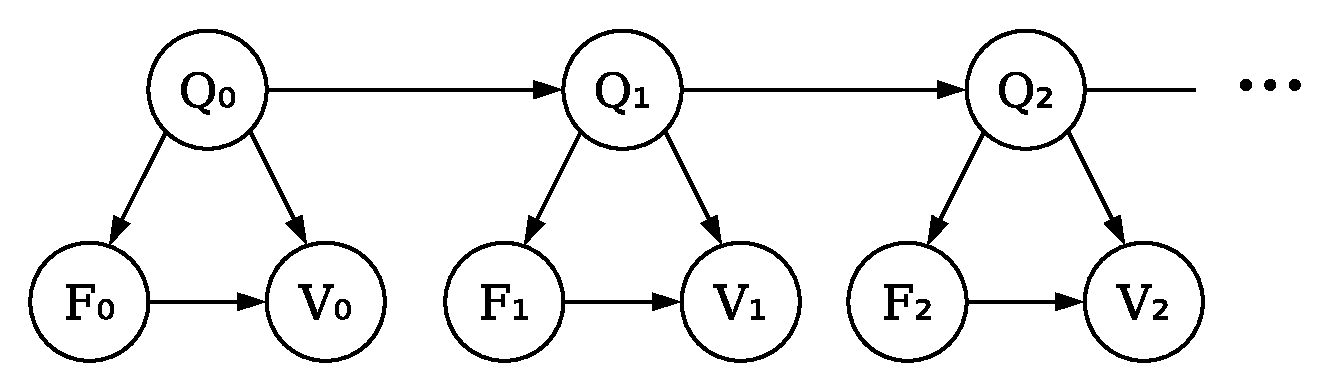
\includegraphics[width=.45\linewidth]{imm}
\caption{Invisible Markov model.}%
\label{fig:imm}
\end{figure}

\begin{definition}
    An IMM cycle is any probable sequence of states that starts and ends with the same state.
    A quiet state is a state that has a non-zero probability of emitting an empty sequence.
    A \textbf{quiet cycle} is any cycle having only quiet states.
\end{definition}

IMMs with no quiet cycles will simplify some calculations as we will see shortly.

\begin{corollary}
Let $M$ be the number of states of the IMM.
If it has no quiet cycles, any sequence of $M$ states will have emitted at least one symbol.
\end{corollary}

The marginal likelihood of $\mathbf z=z_1 .. z_L$ is given by
\begin{align}\label{eq:ml}
    \mathrm{ML}(\mathbf z) = p(V_1=\mathbf z) + p(V_1||V_2=\mathbf z) + \dots,
\end{align}
where $||$ denotes tuple concatenation.
The summation on the right-hand side of the above equation is unbouded if IMM is allowed to have
quiet cycles.
On the other hand, if IMM has no quiet cycles, the marginal likelihood of $\mathbf z=z_1 .. z_L$
can be given by
\begin{align*}
    \mathrm{ML}(\mathbf z) =
    p(V_1=\mathbf z) + p(V_1||V_2=\mathbf z) + \dots + p(V_1||V_2||\dots||V_{L\cdot M}=\mathbf z).
\end{align*}

Let $l_n=f_0+f_1+\dots+f_{n-1}$.
Observe that the outcomes of the random variables $F_1, F_2, \dots$ are enough to assign the subsequences
of $\mathbf z$ to the random variables $V_1, V_2, \dots$ in the following sense:
\begin{alignat*}{3}
    p&(V_1=z_1 .. z_{f_1}, V_2=z_{l_2+1} .. z_{l_2+f_2}, \dots, V_n=z_{l_n+1} .. z_{l_n+f_n}&&) =\\
    p&(V_1=z_1 .. z_{f_1}, V_2=z_{l_2+1} .. z_{l_2+f_2}, \dots, V_n=z_{l_n+1} .. z_{l_n+f_n}&&,
        F_1=f_1, F_2=f_2, \dots, F_n=f_n).
\end{alignat*}
We will therefore use the shorter notation
\begin{align*}
    p(V_{1..n}=\mathbf z, F_1=f_1, F_2=f_2, \dots, F_n=f_n)
\end{align*}
instead.
Also note that, if the association between subsequences of $\mathbf z$ with the random variables $V_1, V_2, \dots$ is
not specified, we still need to sum out the possible combinations:
\begin{align*}
    p(V_{1..n}=\mathbf z) = \sum_{f_1,\dots,f_n} p(V_{1..n}=
    \mathbf z, F_1=f_1, F_2=f_2, \dots, F_n=f_n).
\end{align*}

Lets consider the first term of the right-hand side of Eq. \eqref{eq:ml}.
We have
\begin{align*}
    p(V_1=\mathbf z)
        &= \sum_{q_1} p(V_1=\mathbf z, F_1=L \gv Q_1=q_1) p(Q_1=q_1 \gv Q_0=q_0).
\end{align*}
Lets now consider the second term of the right-hand side of Eq. \eqref{eq:ml}.
\begin{align*}
    p(V_{1..2}=\mathbf z)
        &= \sum_{f_1,f_2} p(V_{1..2}=\mathbf z, f_1, f_2)
        = \sum_{f_1,f_2,q_1,q_2} p(V_{1..2}=\mathbf z, f_1, f_2 \gv q_1, q_2) p(q_1, q_2) \\
        &= \sum_{f_1,f_2,q_2} p(V_2=\mathbf z, f_1, f_2 \gv q_2) \sum_{q_1} p(V_1=\mathbf z, f_1 \gv q_1) p(q_2 \gv q_1) p(q_1 \gv q_0)
\end{align*}


\newpage
\newpage

\section{Old model generalisation}

Let $L_t=F_0+F_1+\dots + F_{t-1}$ be the random variable describing the number of emitted symbols right
before the sequence emission by $Q_t$.
Let $S_1, S_2, \dots$ a stochastic process for symbol emission such that $S_t\in\mathcal A$
and
\begin{align*}
    p(s_{l_t+1} .. s_{l_t+f_t}, L_t=l_t, F_t=f_t, V_t=\mathbf v_t)
        = p(s_{l_t+1} .. s_{l_t+f_t}\gv L_t=l_t, F_t=f_t, V_t=\mathbf v_t).
\end{align*}

Let us define an additional stochastic process  associated with a given IMM
(random variables are omitted for didactic reasons whenever appropriate):
\begin{align*}
    p(S_0=\emptyset\gv Q_0=q_0)
        &=1\\
    p(s_1 .. s_{f_1},f_1,q_1)
        &= p(s_1 .. s_{f_1}\gv f_1,q_1)p(f_1,q_1) = p(s_1 .. s_{f_1}\gv f_1,q_1)p(f_1\gv q_1)p(q_1)\\
    p(s_1 .. s_{f_1+f_2},f_1,f_2,q_1,q_2)
        &= p(s_{f_1+1} .. s_{f_1+f_2}\gv f_1, f_2, q_2)p(s_1 .. s_{f_1}, f_1, f_2, q_1, q_2)\\
        &= p(s_{f_1+1} .. s_{f_1+f_2}\gv f_1, f_2, q_2)p(s_1 .. s_{f_1}\gv f_1, q_1) p(f_1, f_2, q_1, q_2)\\
        &= p(s_{f_1+1} .. s_{f_1+f_2}\gv f_1, f_2, q_2)p(s_1 .. s_{f_1}\gv f_1, q_1) p(f_1\gv q_1) p(f_2\gv q_2)p(q_2\gv q_1)p(q_1)
\end{align*}

\begin{figure}[htbp]
\centering
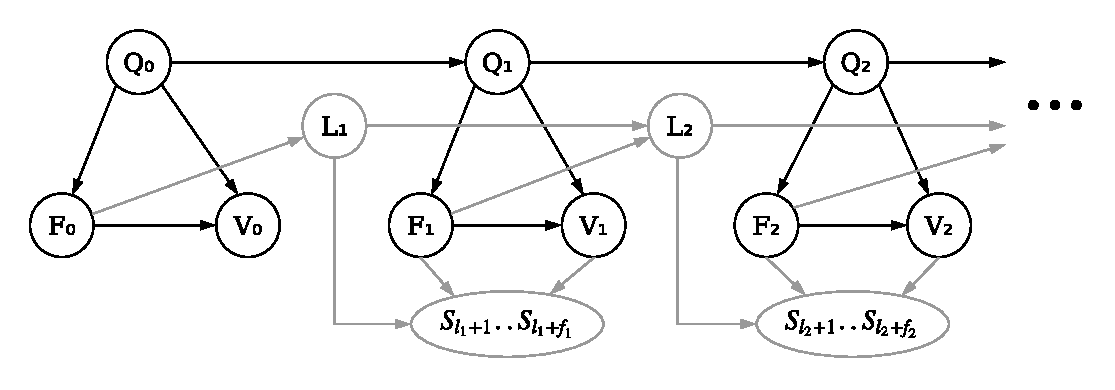
\includegraphics[width=.6\linewidth]{imm-s}
\caption{Invisible Markov model with symbol emission stochastic process.}%
\label{fig:imm-s}
\end{figure}

Let $L_t=F_0+F_1+\dots + F_{t-1}$, be the random variable describing the number of emitted symbols right
before the sequence emission by $Q_t$.
We define
\begin{align*}
    p(S_{l_t+1}=s_{l_t+1}, \dots, S_{l_t+f_t}=s_{l_t+f_t} \gv L_t=l_t, F_t=f_t, Q_t=q_t) =
                                p(V_t=(s_{l_t+1}, \dots, s_{l_t+f_t}) \gv F_t=f_t, Q_t=q_t).
\end{align*}
Given an IMM, we define the marginal likelihood of a sequence $\mathbf z = z_1z_2\dots z_L$
as being
\begin{align*}
    p(S_1=z_1, \dots, S_L=z_L) = \sum\limits_{\substack{q_1..q_N \\ f_1..f_N}}
        p(S_1=z_1, \dots, S_L=z_L, Q_1=q_1, F_1=f_1, \dots, Q_N=q_N, F_N=f_N),
\end{align*}
subject to $L=l_N+f_N$.\footnote{It might be a good moment to talk about degenerate IMM: when there is silent states cycle and/or
there are states with unbounded sequence lengths.}

Silent and non-silent HMM states are particular cases of IMM states that emit sequences of length zero and one,
respectively.

% \begin{align*}
%     p(S_{i_t}=s_{i_t}, S_{i_t+1}=s_{i_t+1}, \dots, S_{i_t+f_t-1}=s_{i_t+f_t-1} &| I_t=i_t, F_t=f_t, Q_t=q_t) =\\
%                                             &p(V_t=(s_{i_t}, s_{i_t+1}, \dots, s_{i_t+f_t-1}) | F_t=f_t, Q_t=q_t).
% \end{align*}

% \section{Old model generalisation}

% The standard HMM description (Def.~\ref{def:hmm}) is usually extended to account for states that do not emit symbols.
% Those states are referred to as silent states and are useful to describe a missing alignment position, for example.
% This section goes a step further by defining an alternative Markov model that accounts for states that instead
% emit sequence of symbols of variable length.

% \begin{definition}
% Let $\mathcal A$ be a finite set of symbols.
% Let $Q_1, Q_2, \dots$ be a Markov process and $F_1, F_2, \dots$ be a stochastic process for which
% \begin{equation*}
%     p(F_t\in\field{N}\gv Q_1=q_1, Q_2=q_2, \dots, Q_t=q_t) = p(F_t\in\field{N}\gv Q_t=q_t).
% \end{equation*}
% Let $V_1, V_2, \dots$ be a stochastic process for which
% \begin{equation*}
%     p(V_t\in\mathcal A^{f_t}\gv Q_1=q_1, F_1=f_1, Q_2=q_2, F_2=f_2, \dots, Q_t=q_t, F_t=f_t)
%         = p(V_t\in\mathcal A^{f_t}\gv Q_t=q_t, F_t=f_t).
% \end{equation*}
% The triplet $(Q_t, F_t, V_t)$ is an invisible Markov model (IMM) with alphabet $\mathcal A$.
% \end{definition}

% Silent and non-silent states are particular cases of IMM states that emit sequences of length zero and one,
% respectively.
% IMM reduces to the standard HMM if $p(F_t=1\gv Q_t=q_t)$ for every $t$.
% Fig.~\ref{fig:imm} illustrates a probabilistic graphical model for IMM.

% Let us define an additional stochastic process $S_1, S_2, \dots$ associated with a given IMM as follows.
% Let $L_t=F_1+\dots + F_{t-1}$, for which $L_1 = 0$, be the random variable describing the number of emitted symbols right
% before the sequence emission by $Q_t$.
% We define
% \begin{align*}
%     p(S_{l_t+1}=s_{l_t+1}, \dots, S_{l_t+f_t}=s_{l_t+f_t} \gv L_t=l_t, F_t=f_t, Q_t=q_t) =
%                                 p(V_t=(s_{l_t+1}, \dots, s_{l_t+f_t}) \gv F_t=f_t, Q_t=q_t).
% \end{align*}
% Given an IMM, we define the marginal likelihood of a sequence $\mathbf z = z_1z_2\dots z_L$
% as being
% \begin{align*}
%     p(S_1=z_1, \dots, S_L=z_L) = \sum\limits_{\substack{q_1..q_N \\ f_1..f_N}}
%         p(S_1=z_1, \dots, S_L=z_L, Q_1=q_1, F_1=f_1, \dots, Q_N=q_N, F_N=f_N),
% \end{align*}
% subject to $L=l_N+f_N$.\footnote{It might be a good moment to talk about degenerate IMM: when there is silent states cycle and/or
% there are states with unbounded sequence lengths.}

\begin{sidewaysfigure}[ht]
    \centering
    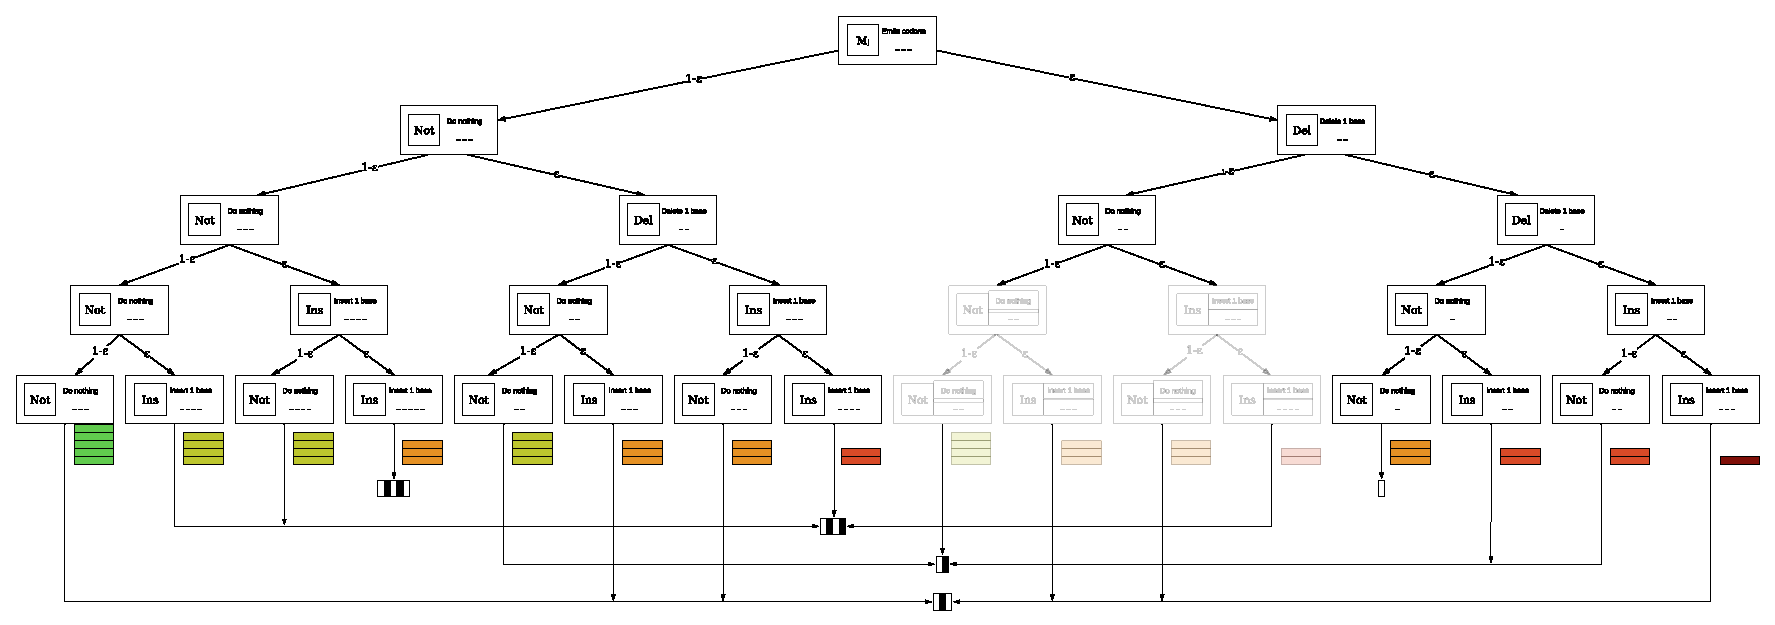
\includegraphics[scale=0.9]{codon-hmm-tree}
    \caption{Matched codon HMM tree.
        The $\eps$-transitions occur infrequently and exist to account for sequence errors.
        The most probably path ends at the first leaf-node from left to right.}\label{fig:codon-hmm-tree}
\end{sidewaysfigure}

\end{document}
